\documentclass[UTF8]{ctexart}
\usepackage{amsmath}
\usepackage{amssymb}
\usepackage{booktabs}
\usepackage{background}
\usepackage{caption, subcaption}
\usepackage{enumitem}
\usepackage{float}
\usepackage{fontspec}
\usepackage{geometry}
\usepackage{pifont}
\usepackage{tikz}
\usepackage{ulem}
\usepackage{xcolor}
\usetikzlibrary{arrows.meta}

\geometry{a5paper, top=0.1cm, left=1cm, right=1cm, bottom=1.1cm}
\setCJKmainfont[BoldFont={汉仪文黑-85W},ItalicFont={方正苏新诗柳楷简体}]{汉仪文黑-55W}
\setfontfamily\Issue{Century Schoolbook}
\newCJKfontfamily\TitleFont{思源宋体 CN Heavy}
\newfontfamily\timesnewroman{Times New Roman}
\captionsetup{font=small, labelfont=bf}
\reversemarginpar

\CTEXsetup[format = {\centering\bfseries\large}, beforeskip = 3pt, afterskip = 3pt]{section}

\colorlet{darkcyan}{cyan!50!black}
\newcommand\Black[1]{\textcolor[gray]{0.3}{#1}}
\newcommand\Brown[1]{\textcolor[HTML]{998A4E}{#1}}
\newcommand\Concept[1]{\colorbox{cyan!10!white}{\textcolor{cyan!40!black}{#1}}}
\newcommand\Emph[1]{\colorbox{violet!10}{\textcolor{violet}{\bfseries #1}}}
\newcommand\Notes[1]{\textcolor{yellow!50!black}{\small #1}}
\newcommand\Example[1]{\textcolor{cyan!70!black}{\small #1}}
\newcommand\pos[1]{\hspace{0pt} \marginpar{\footnotesize\textcolor{yellow!50!black}{\hfill #1}}}

\newcommand\IssueNumber{15}
\newcommand\Date{2023-12-25}
%\newcommand\Contributer{@金光日}
\newcommand\Subject{大学物理 A2}


\begin{document}
\backgroundsetup{contents=
\includegraphics{示例.png}, center, scale=1, angle=0, opacity=1}
\BgThispage
\begin{center}
{\scriptsize\Issue \textcolor[HTML]{C8BA83}{WEEKLY TIPS}}

{\Huge\bfseries\TitleFont \Black{知\ 识\ 小\ 料}}

\vspace{-0.1cm}
{\footnotesize \Brown{「电计 2203 班」周常规知识整理共享}}
\end{center}

\vspace{-0.5cm}

\begin{figure}[H]
\hspace{1cm}
\begin{minipage}[t]{0.3\textwidth}
\centering
    \Brown{ISSUE.}

    \vspace{-0.6cm}
    \Huge \Issue\slshape\bfseries\Black{\IssueNumber}
\end{minipage}
\hfill
\begin{minipage}[t]{0.35\textwidth}
\centering
    \Brown{日期:\Date} \\
%\vspace{-0.1cm}
%    \Brown{贡献者:\Contributer} \\
\vspace{-0.1cm}
    \Brown{学科:\Subject} \\
\end{minipage}
\hspace{0.8cm}
\end{figure}

{
\begin{figure}[htb]
\begin{minipage}[t]{0.74\textwidth}
    \color{cyan!50!black}
    \vspace{0pt}
    对处于 $n=4$ 状态的氢原子,求:

    \begin{enumerate}
    \color{cyan!50!black}
      \item 轨道角动量 $L$ 的最大值和轨道角动量分量 $L_z$ 的最小绝对值(用 $\hbar$ 表示);
      \item 轨道角动量 $\vec{L}$ 与 $z$ 轴的最小夹角,并在右图标示出来。
    \end{enumerate}
\end{minipage}
\begin{minipage}[t]{0.25\textwidth}
\color{cyan!50!black}
\vspace{0pt}
\centering
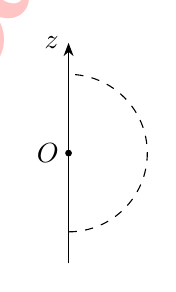
\begin{tikzpicture}
    \draw[->, >=Stealth] (0,-1.4) -- (0,1.4) node[left] {$z$};
    \draw[dashed] (0,-1) arc (-90:90:1);
    \filldraw (0,0) circle (1pt) node[left] {$O$};
\end{tikzpicture}
\end{minipage}
\end{figure}
}

\vspace{-0.8cm}

【解答】
\begin{enumerate}[itemsep=0pt, parsep=0pt]
  \item 主量子数 $n=4$,则角量子数 $l=0,1,2,3$,磁量子数 $m=0,\pm 1,\pm 2,\pm 3$。由
  \begin{equation*}
    L=\sqrt{l(l+1)}\cdot \hbar,\qquad L_z = m \hbar
  \end{equation*}

  取 $l=3$,则 $L_{\max}=\sqrt{3\times 4}\cdot \hbar = 2\sqrt{3}\hbar$;取 $m=0$,则 $|L_z|_{\min}=0$。

  \item 由下图左部分,要使夹角最小,则需 $L_z$ 最大,取 $3\hbar$(或 $-3\hbar$)。
  \begin{equation*}
    \theta = \arccos \dfrac{L_z}{L} = \arccos\dfrac{3\hbar}{2\sqrt{3}\hbar} = 30^\circ
  \end{equation*}
\end{enumerate}

%\newpage
%\backgroundsetup{contents=
\includegraphics{下半示例.png}, center, scale=1, angle=0, opacity=1}
%\BgThispage

\begin{figure}[htb]
\begin{minipage}[t]{0.5\textwidth}
\centering
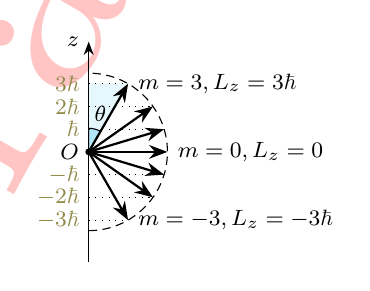
\begin{tikzpicture}[>=Stealth, font=\footnotesize]
    \fill[fill=cyan!10] (0,0) -- (0, 0.866) -- (0.5, 0.866) -- cycle;
    \filldraw[fill=cyan!30] (0,0) -- (0,0.3) arc (90:60:0.3) node[above]{$\theta$} -- cycle;
    \draw[->] (0,-1.4) -- (0,1.4) node[left] {$z$};
    \draw[densely dashed] (0,-1) arc (-90:90:1);
    \draw[dotted] (0, 0.288) -- (0.957, 0.288); % \sqrt{6}/3
    \draw[dotted] (0, 0.577) -- (0.816, 0.577); % *2
    \draw[dotted] (0, 0.866) -- (0.5, 0.866); % *3
    \draw[dotted] (0, -0.288) -- (0.957, -0.288); % \sqrt{6}/3
    \draw[dotted] (0, -0.577) -- (0.816, -0.577); % *2
    \draw[dotted] (0, -0.866) -- (0.5, -0.866); % *3
    \draw[->, thick] (0,0) -- (0.5, -0.866) node[right] {$m=-3,L_z = -3\hbar$};
    \draw[->, thick] (0,0) -- (0.816, -0.577) ;
    \draw[->, thick] (0,0) -- (0.957, -0.288) ;
    \draw[->, thick] (0,0) -- (0.957, 0.288) ;
    \draw[->, thick] (0,0) -- (0.816, 0.577) ;
    \draw[->, thick] (0,0) -- (0.5, 0.866) node[right] {$m=3,L_z = 3\hbar$};
    \draw[->, thick] (0,0) -- (1,0) node[right] {$m=0,L_z = 0$};
    \filldraw (0,0) circle (1pt) node[left] {$O$};
    \foreach \i in {-3,-2,2,3} 
        \node[left, yellow!50!black] at (0, 0.288*\i) {$\i \hbar$};
    \node[left, yellow!50!black] at (0, 0.288) {$\hbar$};
    \node[left, yellow!50!black] at (0,-0.288) {$-\hbar$};
\end{tikzpicture}
\end{minipage}
\begin{minipage}[t]{0.5\textwidth}
\centering
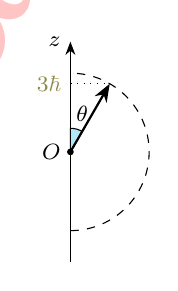
\begin{tikzpicture}[>=Stealth, font=\footnotesize]
    \filldraw[fill=cyan!30] (0,0) -- (0,0.3) arc (90:60:0.3) node[above]{$\theta$} -- cycle;
    \draw[->, >=Stealth] (0,-1.4) -- (0,1.4) node[left] {$z$};
    \draw[dashed] (0,-1) arc (-90:90:1);
    \filldraw (0,0) circle (1pt) node[left] {$O$};
    \draw[dotted] (0, 0.866) -- (0.5, 0.866); % *3
    \draw[->, thick] (0,0) -- (0.5, 0.866);
    \node[left, yellow!50!black] at (0,0.866) {$3\hbar$};
\end{tikzpicture}
\end{minipage}
\end{figure}

\textcolor{cyan!80!black}{【结论】1. $L_{\max}= 2\sqrt{3}\hbar$,$|L_z|_{\min}=0$;2. $\theta=30^\circ$,上图右部分为标示。}

\textcolor{cyan!80!black}{【点评】这题考察了三个量子数的关系:主量子数 $n$、角量子数 $l$ 、磁量子数 $m$ 。角量子数要小于主量子数,而磁量子数的绝对值不超过角量子数。把这一关系记下,并懂得角动量量子化的公式,就可以解出此题。}

\end{document} 